\newpage

\section{Implementation}
The WALE model has been implemented initially in the D3Q27 Matrix code developed in the Institute of Computational modelling in Civil Engineering. This code uses two set of arrays to store the distribution functions and to exchange the post-collision distribution functions every time-step. The WALE model implementation requires the computation of the strain rate tensor and the vorticity rate tensor, which requires the information of the velocity gradients. The velocity gradients have been computed using the finite differences. The macroscopic velocity computed from the distribution functions are used to compute the velocity gradients in every time-step. Apart from the WALE model implementation the topic on the conditioning of the WALE model equation will be discussed here. Towards the end of the section the numerical results of the Taylor green vortex simulations will be compared to the analytical solution to confirm the validity of the eddy-viscosity obtained from the WALE model.

\subsection{Discretisation}
Several velocity gradients i.e. $\partial u_i/\partial x_i$ and $\left(\partial u_i/\partial x_j + \partial u_j/\partial x_i\right)$ are directly available from the Cumulant LB solver~\cite{geier:parameter}. The computation of the strain rate tensor can be easily carried out with those available gradients. But the available information of the velocity gradients was not enough to compute the rotation rate tensor i.e. $\left(\partial u_i/\partial x_j - \partial u_j/\partial x_i\right)$. Since the vorticity calculations had to be  performed using the finite difference method, it was decided to compute the velocity gardients using the finite difference method. \emph{Weickert et.al}~\cite{weickert:LES} implemented the WALE model in the MRT LB framework and they have computed the velocity gradients using the finite differences. 

The purpose of the SGS models is to dissipate the resolved turbulent fluctuations~\cite{davidson}. When finite differences are used in combination with the LES method great care has to be taken to choose the non-dissipative finite difference scheme. This is done to avoid the masking effect of the numerical dissipation on to the dissipation introduced by the SGS models. Taking that into consideration a central difference scheme was chosen to compute the velocity gradients.\\\\
%
\textbf{Treatment of velocity gradients near the boundaries}

In order to avoid the fluid nodes, near the boundaries, accessing the non-fluid nodes due to the central differencing, forward differences and backward differences were used at the respective boundaries to compute the velocity gradients. Fig.(\ref{Finite differences bound}) shows a cuboid marked with the red dots at the inlet, front and the bottom face. The first set of fluid nodes near these faces use forward difference to compute the velocity gradients and the first set of fluid nodes at the exit, top and back faces use backward differences to compute the gradients along the respective directions. Rest fluid nodes used central differences.

\begin{figure}[b]
\centering
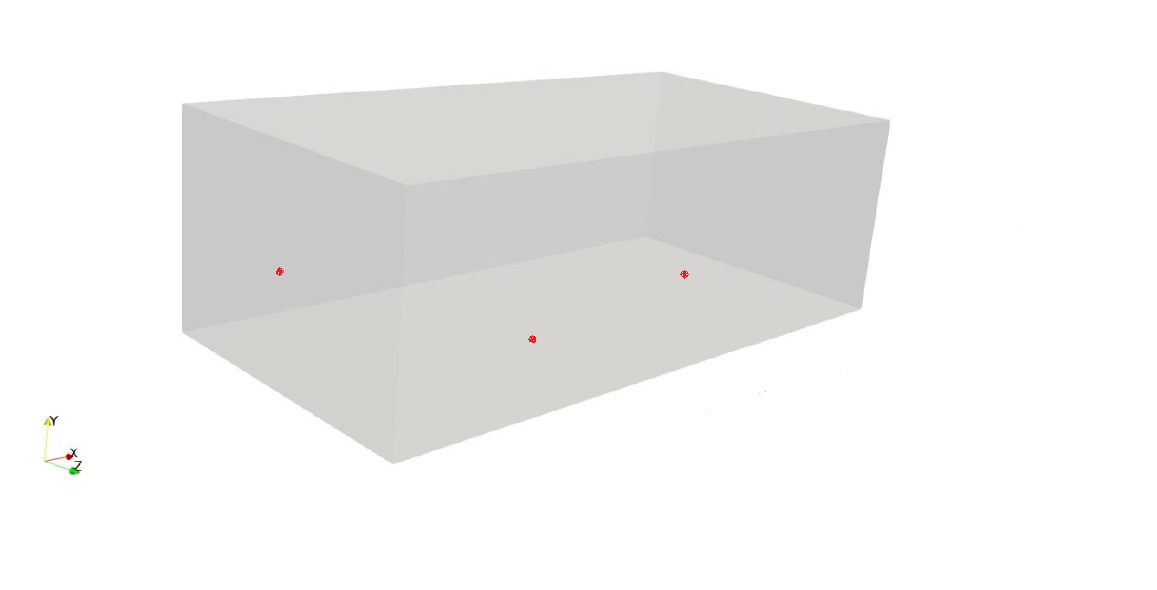
\includegraphics[width=8cm]{04_Implementation/figur/3D_Domain_gradients.png}
\label{Finite differences bound}
\caption{Cuboid representing a channel}
\end{figure}
\subsection{Implementation of eddy viscosity contribution}

The WALE model has been implemented in the LB kernel itself "LB\_Kernel\_2SOD". Few other variations were tried but they required thread synchronisation which is not optimal to do in terms of the efficiency. Hence, it was implemented in the kernel itself. An additional viscosity called eddy viscosity $\left(\nu_t\right)$ has to be introduced in to the solver to model the turbulence. This is given by:
%
\begin{equation}
\label{Eddy viscosity}
\nu_t = \left(C_W \Delta_x \right)^2 \overline{OP}
\end{equation}
\subsection{Taylor-Green vortex simulations}
%
where $C_W$ is the model constant and is
\begin{figure}[h]
%\centering
\begin{minipage}[b]{0.5\textwidth}
\subfigure[global coordinates]{
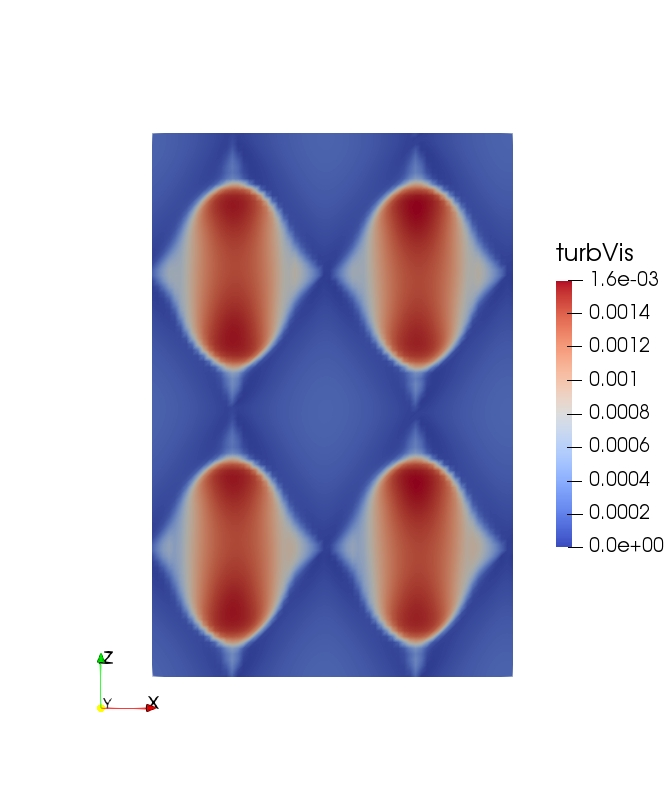
\includegraphics[width=6.7cm]{04_Implementation/figur/nutSimulation_latex_64.jpg}}
\end{minipage}
\end{figure}
%
